\chapter{要素技術}
\label{chap:elemental}
本章では,本研究に関連する要素技術を述べる
\section{メトリックマップに基づくナビゲーション}
メトリックマップに基づくナビゲーションについて述べる.
このナビゲーションは,LiDARやオドメトリなどのセンサとメトリックマップを用いて,
自己位置推定,経路計画を行い,目的地まで自律移動する.
メトリックマップに基づくナビゲーションには
ROS Navigation stack\cite{ros}がよく用いられている.
ROS Navigation stackは主に下記の3つの機能を提供する.
\begin{quote}
    \begin{itemize}
     \item パーティクルフィルタによって自己位置推定を行うモンテカルロ自己位置推定(MCL)
     \item 障害物認識などの局所的または地図全体の大域的なコスト計算と,その結果に基づく経路計画
     \item 経路に追従する並進速度や角速度などの速度指令
    \end{itemize}
   \end{quote}
\figref{fig:nav}にROS Navigation stackによるメトリックマップに基づく
ナビゲーションの様子を示す.
本論文では,図中の赤の経路を追従することを経路追従と呼ぶ.
% 本論文では,Navigation stackをこの模倣学習やデータセットの作成に使用している.
% \vspace{5zh}
\begin{figure}[htbp]
    \centering
     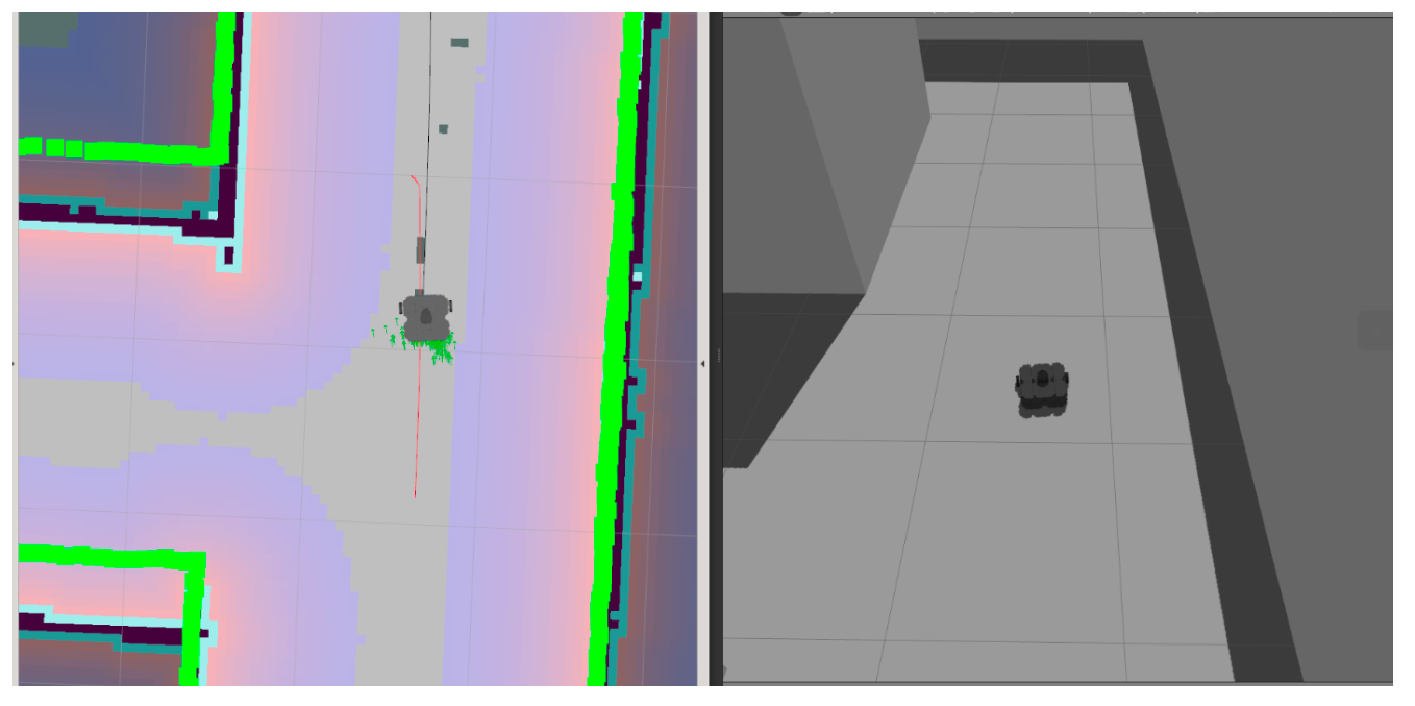
\includegraphics[width=100mm]{images/pdf/nav.pdf}
     \caption{Metric map based navigation (Quoted from\cite{shimada2020})}
     \label{fig:nav}
\end{figure}
岡田らの従来手法,本論文で述べる視覚に基づくナビゲーションでは,
このROS Navigation stackによる経路追従行動を模倣する.
% \section{深層学習}
% \subsection{教師あり学習}
% 教師あり学習は,機械学習の一種であり,
% データセットと呼ばれる
% ラベル付きのデータの集合を使用してモデルを訓練する手法である.
% データセットには,入力データとそれに対応する正解(ラベル)が含まれている.
% モデルはデータセットを利用して,正解となる出力を得られるように学習を行っていく.

% \clearpage
% \subsection{end-to-end学習}
% \ref{fig:e2e}に示すように,入力されるデータから目的の出力を得るために必要なデータを得るために必要な
% 他段階の処理をニューラルネットワークを用いて直接学習する手法である.
% 自律移動を例に述べる.
% 人物や障害物などの物体認識,走行レーンの検出,
% 経路計画,ステアリング制御などの複数個のタスクを解く必要があるが, 
% end-to-end学習では先程のタスクを人間が直接設定せずに
% カメラ画像をニューラルネットワークに入力することで,
% 直接ステアリング操作を学習する.
% \begin{figure}[htbp]
%     \centering
%      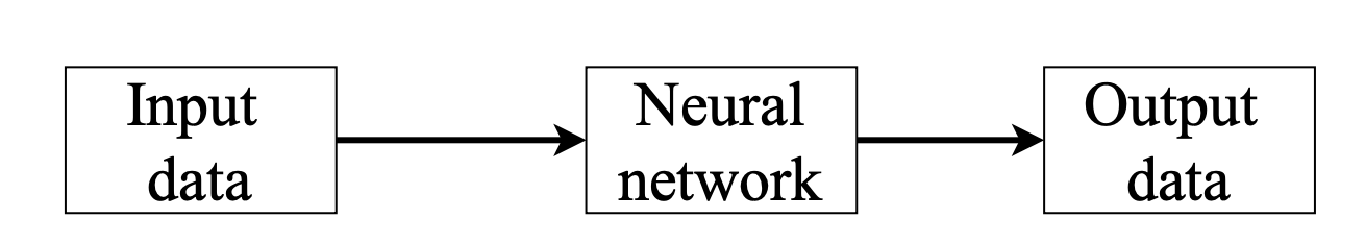
\includegraphics[width=90mm]{images/pdf/e2e.pdf}
%      \caption{Structure of end-to-end learning}
%      \label{fig:e2e}
% \end{figure}

\clearpage
% \section{視覚と行動のend-to-end学習により経路追従行動を
% オンラインで模倣する手法}
% 本論文のベースとなる
% 岡田らの従来手法について述べる.
% この手法では,メトリックマップに基づくナビゲーションの経路追従行動をend-to-end学習により,
% 視覚を入力とした行動へ模倣する.
% これにより,視覚に基づくナビゲーションを獲得できる.
% 手法に基づいて構築されたシステムをに示す.

% 学習器の訓練時,LiDARやオドメトリを入力とするメトリックマップに基づく
% ルールベース制御器を用いて,設定した経路を追従する.
% その際,ロボットに取り付けた,カメラから得たRGB画像とルールベース制御器が出力する
% ヨー方向の角速度をペアとして0.2秒の周期でデータセットへ加える.
% 次にデータセットから,バッチサイズを8として教師データを抽出し,0.2秒の周期で
% end-to-end学習する.
% このデータセットへのデータの追加から学習までの1連の流れを1ステップとしている.
% カメラ画像の収集には,3つのカメラを用いる.
% 左右のカメラ画像に対するヨー方向の角速度は,経路に戻るようなオフセット(\(\pm0.2\)rad/s)を加える.
% ロボットの制御は,メトリックマップに基づくルールベース制御器と視覚を入力とする学習器
% の2つを切り替えることが可能である.

% 学習器の訓練後は,中央のカメラから得たRGB画像を基に
% 学習器が出力するヨー方向の角速度を用いて経路を追従する.
% この時,並進速度は0.2m/sの一定の値を用いる.

% \begin{figure}[htbp]
%     \centering
%      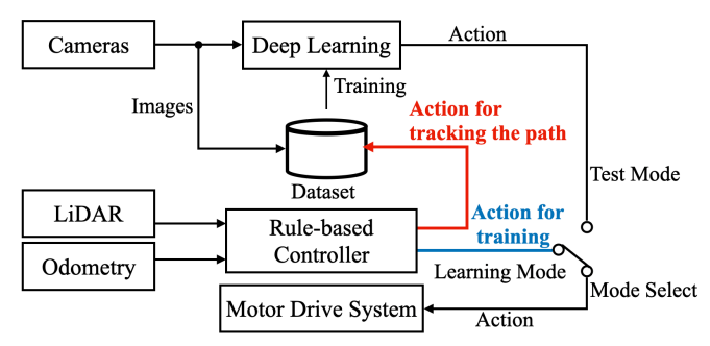
\includegraphics[width=110mm]{images/pdf/okada_method_sys.pdf}
%      \caption{Structure of the Okada and others proposed system (Quoted from\cite{okada2020})}
%      \label{fig:okada_sys}
% \end{figure}
% \clearpage
% この岡田らの従来手法は,ルールベース制御器を教師データの収集に用いることで,
% データセットを収集に人間の操作が不要あること,
% \figref{fig:robo_ac}に示すように学習のデータセットに加える行動と
% 学習時にロボットを制御する行動を別々に
% 扱うことで,常に経路に戻る行動のみをデータセットに追加できるといった特長がある.
% \begin{figure}[htbp]
%     \centering
%      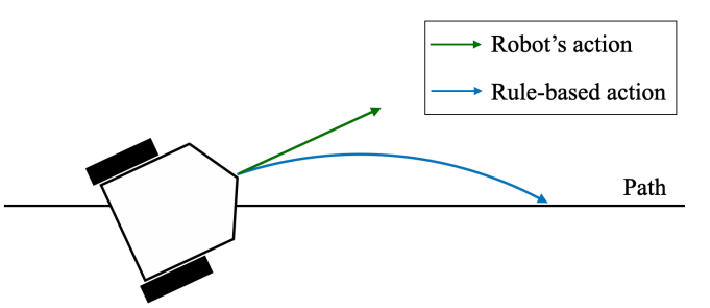
\includegraphics[width=100mm]{images/pdf/robo_action.pdf}
%      \caption{Rule-based actions
%      apart from the robot's actions Quoted from\cite{okada2020}}
%      \label{fig:robo_ac}
% \end{figure}

% \figref{fig:okada_net}
% に岡田らの従来手法における学習器のネットワーク構造を示す.
% ネットワークは,入力層 1,畳み込み層 3,全結合層 2,出力層 1 の全7層で構成される.
% 活性化関数としてReLU\cite{relu},最適化アルゴリズムにAdam\cite{adam}
% 損失関数としてはSoftmax-cross-entropyを用いる.
% 学習器は入力を64x48のRGB画像データ,出力をロボットのヨー方向の角速度として
% end-to-end学習する.
% \begin{figure}[htbp]
%     \centering
%      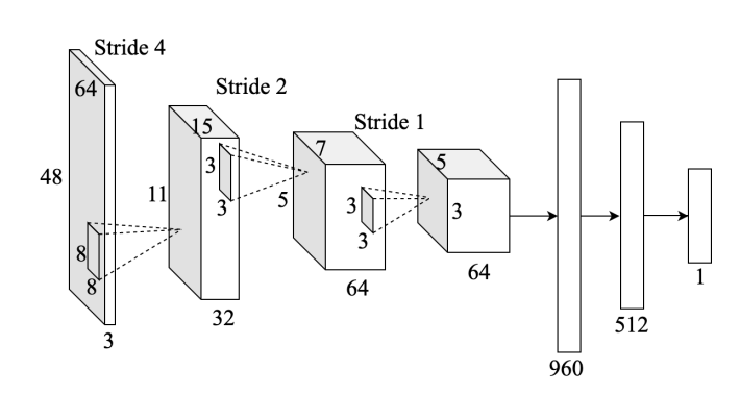
\includegraphics[width=100mm]{images/pdf/okada_network.pdf}
%      \caption{Structure of the network used in the method of Okada and others. (Quoted from \cite{okada2020})}
%      \label{fig:okada_net}
% \end{figure}

% \clearpage
% \section{トポロジカルマップ}
% トポロジカルマップは,環境中のランドマークなどの
% 特徴的な箇所(ノード)とその繋がり(エッジ)によって
% 環境を表現したマップである.
% 島田らは\figref{fig:topo}に示すようなトポロジカルマップの形式\cite{shimada2020}を提案している.
% トポロジカルマップのノードは,通路の特徴的な箇所に配置され,エッジはこれらのノードを
% 接続するように配置されている.
% ノードにはID,通路の特徴(Type),エッジのIDと相対角度(Edge)のデータが含まれている.
% なお,エッジはIDのみをもっている.
% このトポロジカルマップの形式は,人の道案内に関するアンケートにおいて,
% 通路の特徴が多用されたことに基づいて決定された.
% % 該当する位置に配置され,
% % その位置がどのような通路の特徴であるかという情報を
% % 持っている.また,「直進」や「右折」といった~で述べるシナリオの行動から
% % 移動するエッジを選択するために,ノードはエッジのIDと相対角度の情報を
% % 持っている.エッジはノードの接続関係を表すように
% % ノード同士を結んでいる.多くの研究では距離に関する情報を持っていることが
% % 多いが,島田らの形式ではIDのみを持っている.
% % 本稿で用いるトポロジカルマップは,島田らが提案した形式を指す.
% \vspace{5zh}
% \begin{figure}[htbp]
%     \centering
%      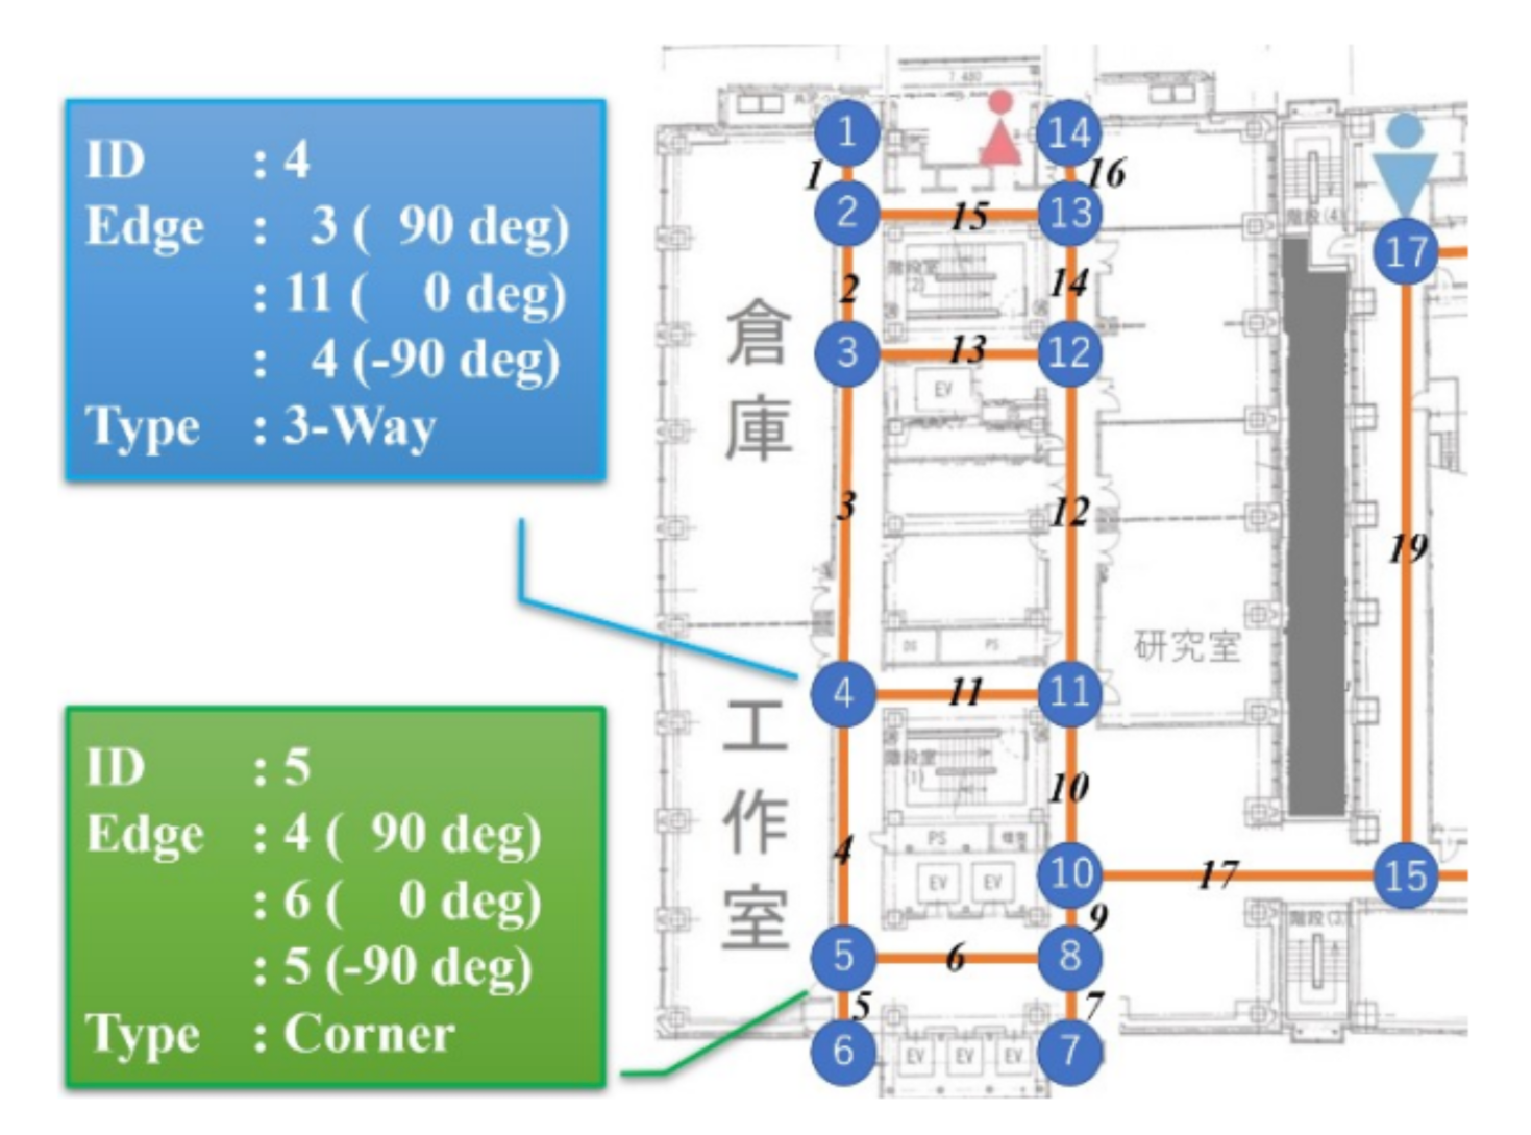
\includegraphics[width=130mm]{images/pdf/topo.pdf}
%      \caption{Topological map format proposed by Shimada and others (Quoted from\cite{shimada2020})}
%      \label{fig:topo}
% \end{figure}
% \clearpage
% \section{シナリオ}
% シナリオはトポロジカルマップ上での,目的地までの経路を単語の組み合わせで表現したものである,
% シナリオは「次の角」や「突き当たり」のような「条件」と「直進」,「右折」のような「行動」の組み合わせにより作成される.
% このシナリオの形式は,トポロジカルマップと同様に
% 人の道案内に関するアンケートで得た,
% 「次の角まで」のような「条件」と「左折」などの「行動」を組み合わせているという
% 情報を基に決定している,
% 例えば,\figref{fig:scenario01}に示すような経路をシナリオで表すと,「3番目の三叉路まで直進.停止」となる.
% \vspace{3zh}
% \begin{figure}[htbp]
%     \centering
%      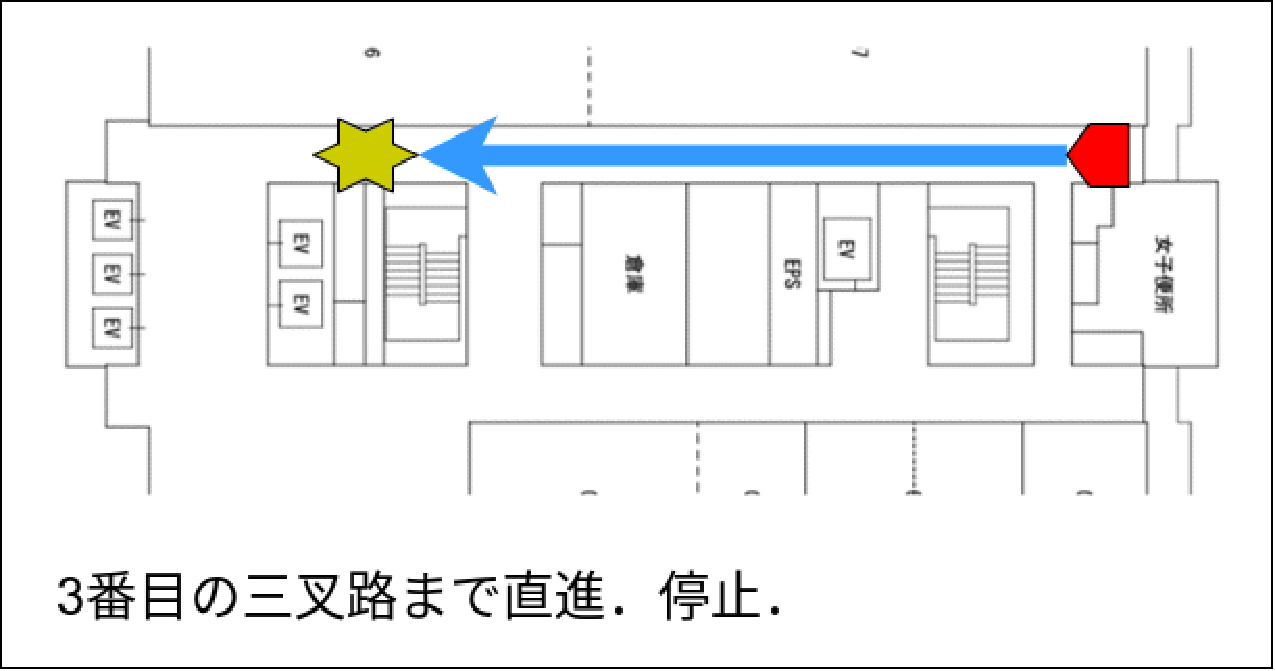
\includegraphics[width=110mm]{images/pdf/scenario/scenario01.pdf}
%      \caption{Example scenarios (Quoted from \cite{haruyama2023})}
%      \label{fig:scenario01}
% \end{figure}